\documentclass[a4paper,14pt,oneside,final]{extarticle}
\usepackage[top=2cm, bottom=2cm, left=3cm, right=1cm]{geometry}
\usepackage{scrextend}

\usepackage[T2A,T1]{fontenc}
\usepackage[ukrainian,russian,english]{babel}
\usepackage{tempora}
\usepackage{fontspec}
\setmainfont{tempora}

% Зачем: Отключает использование изменяемых межсловных пробелов.
% Почему: Так не принято делать в текстах на русском языке.
\frenchspacing

\usepackage{indentfirst}
\setlength{\parindent}{1.25cm}
\renewcommand{\baselinestretch}{1.5}

% Header
\usepackage{fancyhdr}
\pagestyle{fancy}
\fancyhead{}
\fancyfoot{}
\fancyhead[R]{\small \selectfont \thepage}
\renewcommand{\headrulewidth}{0pt}

% Captions
\usepackage{chngcntr}
\counterwithin{figure}{section}
\counterwithin{table}{section}
\usepackage[tableposition=top]{caption}
\usepackage{subcaption}
\DeclareCaptionLabelFormat{gostfigure}{Рисунок #2}
\DeclareCaptionLabelFormat{gosttable}{Таблиця #2}
\DeclareCaptionLabelSeparator{gost}{~---~}
\captionsetup{labelsep=gost}
\captionsetup[figure]{labelformat=gostfigure}
\captionsetup[table]{labelformat=gosttable}
\renewcommand{\thesubfigure}{\asbuk{subfigure}}

% Sections
\usepackage[explicit]{titlesec}
\newcommand{\sectionbreak}{\clearpage}

\titleformat{\section}
  {\centering}{\thesection \quad}{0pt}{\MakeUppercase{#1}}
\titleformat{\subsection}[block]
  {\bfseries}{\thesubsection \quad #1}{0cm}{}

\titlespacing{\section} {0cm}{0cm}{21pt}
\titlespacing{\subsection} {\parindent}{21pt}{0cm}
\titlespacing{\subsubsection} {\parindent}{0cm}{0cm}

% Lists
\usepackage{enumitem}
\renewcommand\labelitemi{--}
\setlist[itemize]{noitemsep, topsep=0pt, wide}
\setlist[enumerate]{noitemsep, topsep=0pt, wide, label=\arabic*}
\setlist[description]{labelsep=0pt, noitemsep, topsep=0pt, leftmargin=2\parindent, labelindent=\parindent, labelwidth=\parindent, font=\normalfont}

% Toc
\usepackage{tocloft}
\tocloftpagestyle{fancy}
\renewcommand{\cfttoctitlefont}{}
\setlength{\cftbeforesecskip}{0pt}
\renewcommand{\cftsecfont}{}
\renewcommand{\cftsecpagefont}{}
\renewcommand{\cftsecleader}{\cftdotfill{\cftdotsep}}

\usepackage{float}
\usepackage{pgfplots}
\usepackage{graphicx}
\usepackage{multirow}
\usepackage{amssymb,amsfonts,amsmath,amsthm}
\usepackage{csquotes}

\usepackage{listings}
\lstset{basicstyle=\footnotesize\ttfamily,breaklines=true}
\lstset{language=Matlab}

\usepackage[
	backend=biber,
	sorting=none,
	language=auto,
	autolang=other
]{biblatex}
\DeclareFieldFormat{labelnumberwidth}{#1}

% Copied from
% https://github.com/cansik/kotlin-latex-listing
% big thanks to him!
\lstdefinelanguage{Kotlin}{
  keywords={package, as, as?, typealias, this, super, val, var, fun, for, null, true, false, is, in, throw, return, break, continue, object, if, try, else, while, do, when, class, interface, enum, object, companion, override, public, private, get, set, import, abstract, vararg, expect, actual, where, suspend, data, internal, dynamic, final, by},
  keywordstyle=\color{NavyBlue}\bfseries,
  ndkeywords={@Deprecated, @JvmName, @JvmStatic, @JvmOverloads, @JvmField, @JvmSynthetic, Iterable, Int, Long, Integer, Short, Byte, Float, Double, String, Runnable, Array},
  ndkeywordstyle=\color{BurntOrange}\bfseries,
  emph={println, return@, forEach, map, mapNotNull, first, filter, firstOrNull, lazy, delegate},
  emphstyle={\color{OrangeRed}},
  identifierstyle=\color{black},
  sensitive=true,
  commentstyle=\color{gray}\ttfamily,
  comment=[l]{//},
  morecomment=[s]{/*}{*/},
  stringstyle=\color{ForestGreen}\ttfamily,
  morestring=[b]",
  morestring=[s]{"""*}{*"""},
}


\newcommand{\labnumber}{3} % third lab
\documentclass[a4paper,14pt,oneside,final]{extarticle}
\usepackage[top=2cm, bottom=2cm, left=3cm, right=1cm]{geometry}
\usepackage{scrextend}

\usepackage[T2A,T1]{fontenc}
\usepackage[ukrainian,russian,english]{babel}
\usepackage{tempora}
\usepackage{fontspec}
\setmainfont{tempora}

% Зачем: Отключает использование изменяемых межсловных пробелов.
% Почему: Так не принято делать в текстах на русском языке.
\frenchspacing

\usepackage{indentfirst}
\setlength{\parindent}{1.25cm}
\renewcommand{\baselinestretch}{1.5}

% Header
\usepackage{fancyhdr}
\pagestyle{fancy}
\fancyhead{}
\fancyfoot{}
\fancyhead[R]{\small \selectfont \thepage}
\renewcommand{\headrulewidth}{0pt}

% Captions
\usepackage{chngcntr}
\counterwithin{figure}{section}
\counterwithin{table}{section}
\usepackage[tableposition=top]{caption}
\usepackage{subcaption}
\DeclareCaptionLabelFormat{gostfigure}{Рисунок #2}
\DeclareCaptionLabelFormat{gosttable}{Таблиця #2}
\DeclareCaptionLabelSeparator{gost}{~---~}
\captionsetup{labelsep=gost}
\captionsetup[figure]{labelformat=gostfigure}
\captionsetup[table]{labelformat=gosttable}
\renewcommand{\thesubfigure}{\asbuk{subfigure}}

% Sections
\usepackage[explicit]{titlesec}
\newcommand{\sectionbreak}{\clearpage}

\titleformat{\section}
  {\centering}{\thesection \quad}{0pt}{\MakeUppercase{#1}}
\titleformat{\subsection}[block]
  {\bfseries}{\thesubsection \quad #1}{0cm}{}

\titlespacing{\section} {0cm}{0cm}{21pt}
\titlespacing{\subsection} {\parindent}{21pt}{0cm}
\titlespacing{\subsubsection} {\parindent}{0cm}{0cm}

% Lists
\usepackage{enumitem}
\renewcommand\labelitemi{--}
\setlist[itemize]{noitemsep, topsep=0pt, wide}
\setlist[enumerate]{noitemsep, topsep=0pt, wide, label=\arabic*}
\setlist[description]{labelsep=0pt, noitemsep, topsep=0pt, leftmargin=2\parindent, labelindent=\parindent, labelwidth=\parindent, font=\normalfont}

% Toc
\usepackage{tocloft}
\tocloftpagestyle{fancy}
\renewcommand{\cfttoctitlefont}{}
\setlength{\cftbeforesecskip}{0pt}
\renewcommand{\cftsecfont}{}
\renewcommand{\cftsecpagefont}{}
\renewcommand{\cftsecleader}{\cftdotfill{\cftdotsep}}

\newcommand{\khpistudentgroup}{КН-34г}
\newcommand{\khpistudentname}{Чепурний~А.~С.}

\newcommand{\khpidepartment}{Програмна інженерія та інформаційні технології управління}
\newcommand{\khpititlewhat}{
	Лабораторна робота №\labnumber \\
	з предмету <<Моделювання систем>>
}
\newcommand{\khpititlewho}{
	Виконав: \\
	\hspace*{\parindent} ст. групи \khpistudentgroup \\
	\hspace*{\parindent} \khpistudentname \\
	Перевірила: \\
	\hspace*{\parindent} ст. в. каф. ПІІТУ \\
	\hspace*{\parindent} Єршова~С.~І. \\
	\hspace*{\parindent} ас. каф. ПІІТУ \\
	\hspace*{\parindent} Литвинова~Ю.~С. \\
}



\lstset{language=Kotlin}
\graphicspath{{figures/}}

\begin{document}
\Ukrainian

\begin{titlepage}

\begin{center}
	МІНІСТЕРСТВО ОСВІТИ І НАУКИ УКРАЇНИ \\
	НАЦІОНАЛЬНИЙ ТЕХНІЧНИЙ УНІВЕРСИТЕТ \\
	«ХАРКІВСЬКИЙ ПОЛІТЕХНІЧНИЙ ІНСТИТУТ» \\[0.5cm]
	Кафедра <<\khpidepartment>> \\
\end{center}

\vspace{6cm}

\begin{center}
	\khpititlewhat
\end{center}

\vspace{3cm}

\begin{addmargin}[10cm]{0cm}
	\khpititlewho
\end{addmargin}

\vspace{\fill}

\begin{center}
	Харків \the\year
\end{center}

\end{titlepage}

\addtocounter{page}{1}

\section*{Проектування програмного забезпечення для моделювання неперервних детермінованих систем}
\subsubsection*{Мета роботи}
Отримати практичні навички архітектурного проектування
програмного забезпечення.
\subsubsection*{Хід роботи}
\begin{enumerate}
\item Визначити стратегію проектування для реалізації програмного забезпечення згідно індивідуального завдання.
\item Розробити моделі для статичного представлення архітектури програмного забезпечення.
\item Розробити моделі для динамічного представлення архітектури програмного забезпечення.
\item Задокументувати розроблені моделі, використовуючи Visual Paradigm for UML.
\item Оформити звіт, який повинен містити обґрунтування вибору архітектури програмного забезпечення, розроблені за допомогою Visual Paradigm for UML моделі структурного та динамічного представлення компонентів системи.
\end{enumerate}

\subsection{Стратегія проектування}
Стратегією проектування було обрано об'єктно-орієнтоване проектування через специфіку фреймворка Android.

\subsection{Моделі для статичного представлення архітектури}
\subsubsection{Діаграми класів і об’єктів}
Діаграми класів і об’єктів використовуються для представлення набору класів і статичних зв'язків між ними.

Діаграма класів представлена на рисунку~\ref{fig:uml_class}.

\begin{figure}[H]
  \centering
    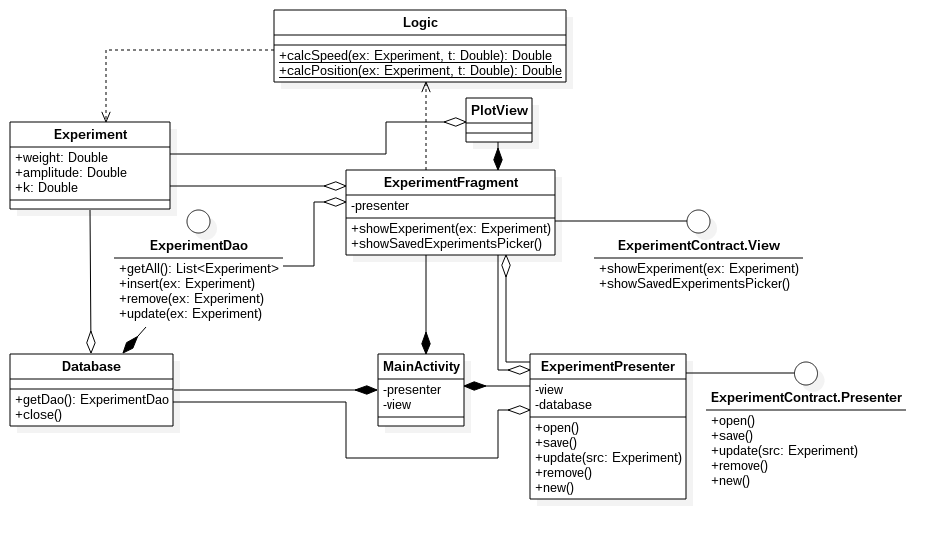
\includegraphics[width=1\textwidth]{uml_class}
  \caption{Діаграма класів}
  \label{fig:uml_class}
\end{figure}

Сутності експерименту відповідає клас \texttt{Experiment}, діаграма об'єктів якого представлена на рисунку~\ref{fig:uml_object_experiment}.

\begin{figure}[H]
  \centering
    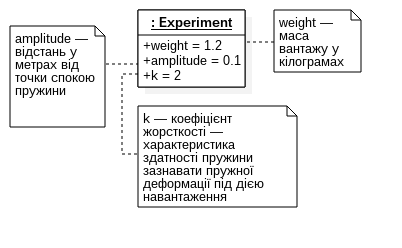
\includegraphics[width=0.6\textwidth]{uml_object_experiment}
  \caption{Діаграма об'єкту \texttt{Experiment}}
  \label{fig:uml_object_experiment}
\end{figure}

\subsubsection{Діаграми компонентів}
Діаграми компонентів або компонентні діаграми у певній мірі аналогічні діаграмам класів, однак, в силу специфіки концепції або поняття компонента, зазвичай, надаються в іншій візуальній формі.

Діаграма компонентів представлена на рисунку~\ref{fig:uml_component}.

\begin{figure}[H]
  \centering
    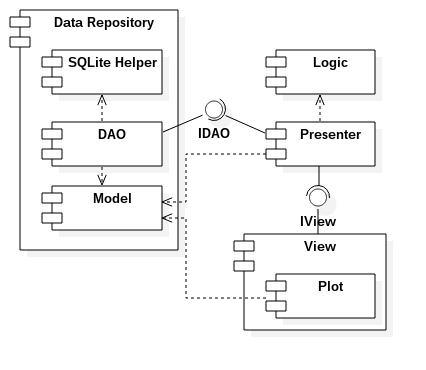
\includegraphics[width=0.7\textwidth]{uml_component}
  \caption{Діаграма компонентів}
  \label{fig:uml_component}
\end{figure}

\subsubsection{Діаграми розгортання}
Діаграми розгортання використовується для представлення (фізичних) вузлів, зв'язків між ними і моделювання інших фізичних аспектів системи.

Діаграма розгортання системи представлена на рисунку~\ref{fig:uml_deployment}.

\begin{figure}[H]
  \centering
    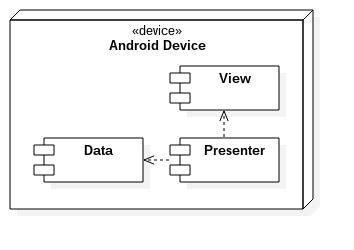
\includegraphics[width=0.5\textwidth]{uml_deployment}
  \caption{Діаграма розгортання}
  \label{fig:uml_deployment}
\end{figure}

\subsubsection{Діаграми сутність-зв’язок}
Діаграми сутність-зв’язок використовується для представлення моделі даних, які зберігаються в процесі роботи інформаційної системи.

Логічна модель даних представлена на рисунку~\ref{fig:erd}.

\begin{figure}[H]
  \centering
    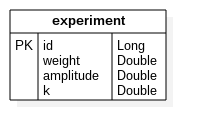
\includegraphics[width=0.3\textwidth]{erd}
  \caption{Діаграма сутність-зв’язок моделі даних}
  \label{fig:erd}
\end{figure}

Модель даних складається з однієї сутності \texttt{experiment}, яка складається з ідентифікатору та фізичних параметрів експерименту.

\subsubsection{Мови опису/визначення інтерфейсу}
Мови опису/визначення інтерфейсу подібні до мов програмування, що не включають можливостей опису логіки системи і призначені для визначення інтерфейсів програмних компонентів (імен та типів експортованих або публікованих операцій).

Опис інтерфейсу \texttt{ExperimentContract.View}:
\lstinputlisting{code/iview.kt}

Опис інтерфейсу \texttt{ExperimentContract.Presenter}:
\lstinputlisting{code/ipresenter.kt}

\subsubsection{Структурні діаграми Джексона}
Структурні діаграми Джексона використовуються для опису структур даних у термінах послідовності, вибору і ітерацій (повторень).

Структурна діаграма Джексона представлена на рисунку~\ref{fig:jackson_structure}.

\begin{figure}[H]
  \centering
    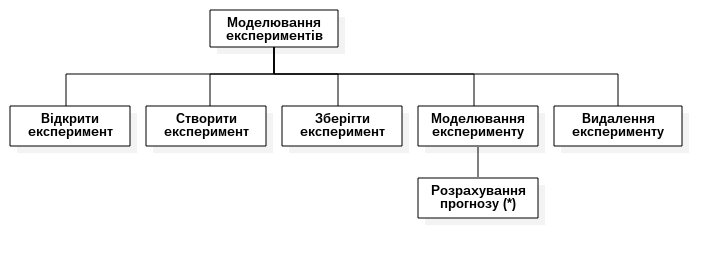
\includegraphics[width=1\textwidth]{jackson_structure}
  \caption{Структурна діаграма Джексона}
  \label{fig:jackson_structure}
\end{figure}

\subsection{Моделі для динамічного представлення архітектури}
\subsubsection{Діаграми діяльності або операцій}
Діаграми діяльності або операцій використовуються для опису потоків робіт і управління.

Діаграма діяльності для створення нового експерименту та його збереження представлена на рисунку~\ref{fig:uml_activity_experiment}.

\begin{figure}[H]
  \centering
    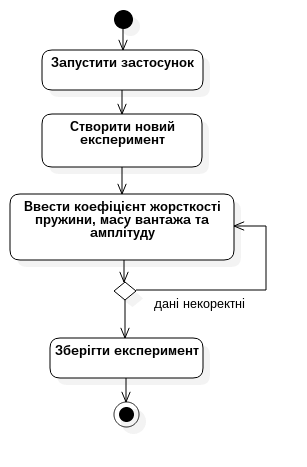
\includegraphics[width=0.4\textwidth]{uml_activity_experiment}
  \caption{Діаграма діяльності для створення та збереження нового експерименту}
  \label{fig:uml_activity_experiment}
\end{figure}

\subsubsection{Діаграми співробітництва}
Діаграми співробітництва показують динамічну взаємодію, що відбувається в групі об'єктів, і приділяють особливу увагу об'єктам, зв'язкам між ними і повідомленням, якими обмінюються об'єкти за допомогою цих зв'язків.

Діаграма співробітництва для створення нового експерименту, його редагування та збереження представлені на рисунках~\ref{fig:uml_communication_experiment_create},~\ref{fig:uml_communication_experiment_edit} та~\ref{fig:uml_communication_experiment_save}.

\begin{figure}[H]
  \centering
    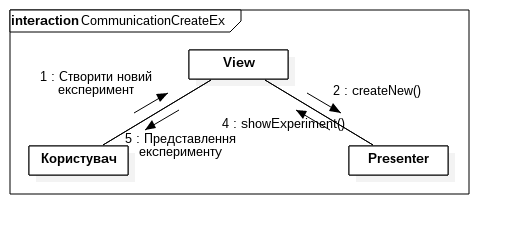
\includegraphics[width=0.8\textwidth]{uml_communication_experiment_create}
  \caption{Діаграма співробітництва для створення нового експерименту}
  \label{fig:uml_communication_experiment_create}
\end{figure}

\begin{figure}[H]
  \centering
    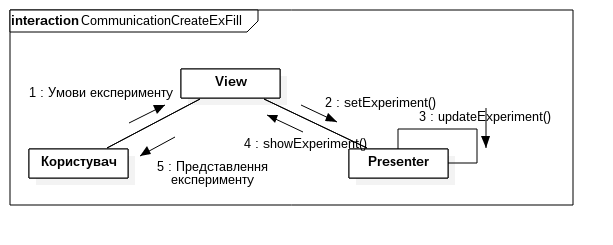
\includegraphics[width=1\textwidth]{uml_communication_experiment_edit}
  \caption{Діаграма співробітництва для редагування експерименту}
  \label{fig:uml_communication_experiment_edit}
\end{figure}

\begin{figure}[H]
  \centering
    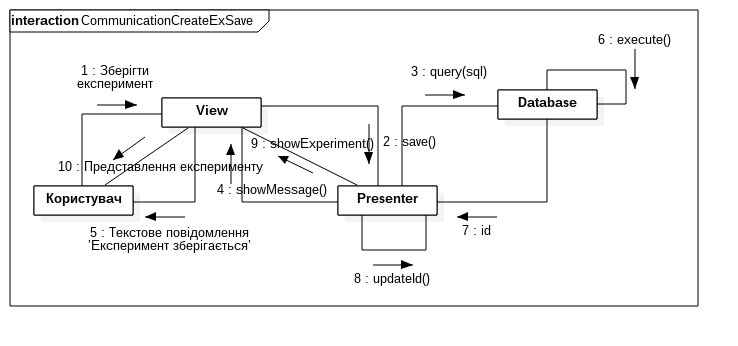
\includegraphics[width=1\textwidth]{uml_communication_experiment_save}
  \caption{Діаграма співробітництва для збереження експерименту}
  \label{fig:uml_communication_experiment_save}
\end{figure}

\subsubsection{Діаграми потоків даних}
Діаграми потоків даних описують потоки даних всередині набору процесів (не в термінах процесів операційного середовища, але в розумінні обміну інформацією в бізнес-контексті).

Діаграма потоків даних представлена на рисунку~\ref{fig:dfd}.

\begin{figure}[H]
  \centering
    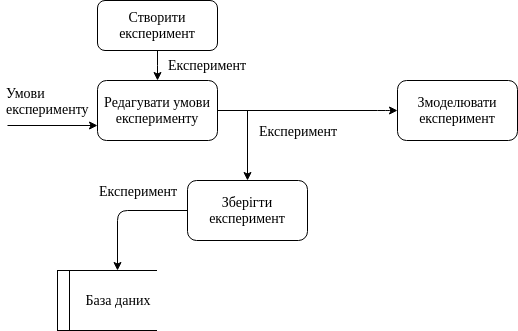
\includegraphics[width=0.8\textwidth]{dfd}
  \caption{Діаграми потоків даних}
  \label{fig:dfd}
\end{figure}

\subsubsection{Блок-схеми і структуровані блок-схеми}
Блок-схеми і структуровані блок-схеми застосовуються для представлення потоків управління (контролю) та пов'язаних операцій.

Блок-схеми класу \texttt{Logic} представлені на рисунку~\ref{fig:uml_flowchart_logic}.

\begin{figure}[H]
  \centering
    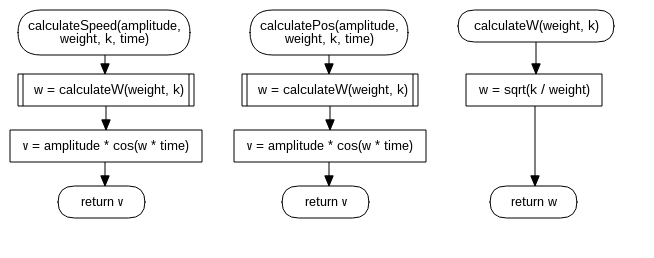
\includegraphics[width=1\textwidth]{uml_flowchart_logic}
  \caption{Блок-схеми класу \texttt{Logic}}
  \label{fig:uml_flowchart_logic}
\end{figure}

\subsubsection{Діаграми послідовності}
Діаграми послідовності використовуються для опису взаємодій всередині групи об'єктів з акцентом на тимчасовій послідовності повідомлень/викликів.

\begin{figure}[H]
  \centering
    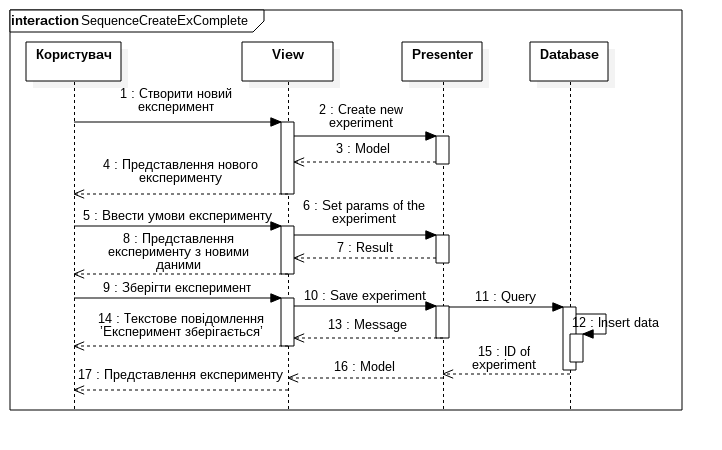
\includegraphics[width=1\textwidth]{uml_sequence_experiment}
  \caption{Діаграми переходу і карти станів}
  \label{fig:uml_sequence_experiment}
\end{figure}

\subsubsection{Діаграми переходу і карти станів}
Діаграми переходу і карти станів застосовуються для опису потоків управління переходами між станами.

На рисунку~\ref{fig:uml_statechart_experiment_edit} представлена діаграма переходів між станами для процесу редагування експерименту.

\begin{figure}[H]
  \centering
    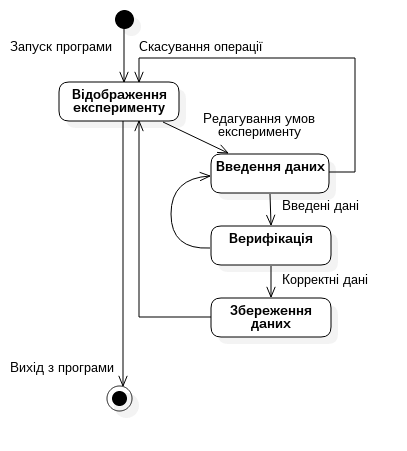
\includegraphics[width=0.6\textwidth]{uml_statechart_experiment_edit}
  \caption{Діаграми переходів між станами для процесу редагування експерименту}
  \label{fig:uml_statechart_experiment_edit}
\end{figure}

\subsubsection{Псевдокод і програмні мови проектування}
Псевдокод і програмні мови проектування використовуються для опису поведінки процедур і методів, в основному на стадії детального проектування; подібні структурним мовам програмування.

Опис класу \texttt{Logic}:
\lstinputlisting{code/logic.kt}

\end{document}
